\documentclass[12pt]{article}   % stay with the familiar article class
\usepackage{reportstyle}        % <— all customisations arrive here
\usepackage{subcaption}
% Make subfigure references appear as 2(a), 2(b)
\captionsetup[subfigure]{labelformat=simple}
\renewcommand\thesubfigure{(\alph{subfigure})}
\DeclareSIUnit{\decade}{dec}

% helper: define only if still undefined
\providecommand{\moduleheader}[1]{}
\providecommand{\titleimage}[1]{}
\providecommand{\titleimageheight}[1]{}

% --- front-matter settings specific to *this* report ---
\title{Analogue Electronics (Project) 4 Simulation Project Report}
\author{Steven \\ s2291752}
\date{\today}
\moduleheader{Analogue Electronics (Project) 4}

% optional image settings
\titleimage{Analogue\_electronics}          % file must be present
\titleimageheight{0.3\textheight}   % tweak height

\begin{document}
	
	\maketitle
	
	\section{Exercise 1: Transistor parameter extraction}
	
	In this section of exercise, I'm going to simulate the transistors in Cadence Virtuoso, and extract some parameters from the simulation result using a simple transistor model. Finally, I'll analysis some questions based on the extracted parameters and the theoretical model. The first simulation is a plot of a group of $I_d$ against $V_{DS}$ under different value of $V_{GS}$, this is shown in Figure \ref{fig:groupIdVds}.

	\begin{figure}[htbp]
		\centering
		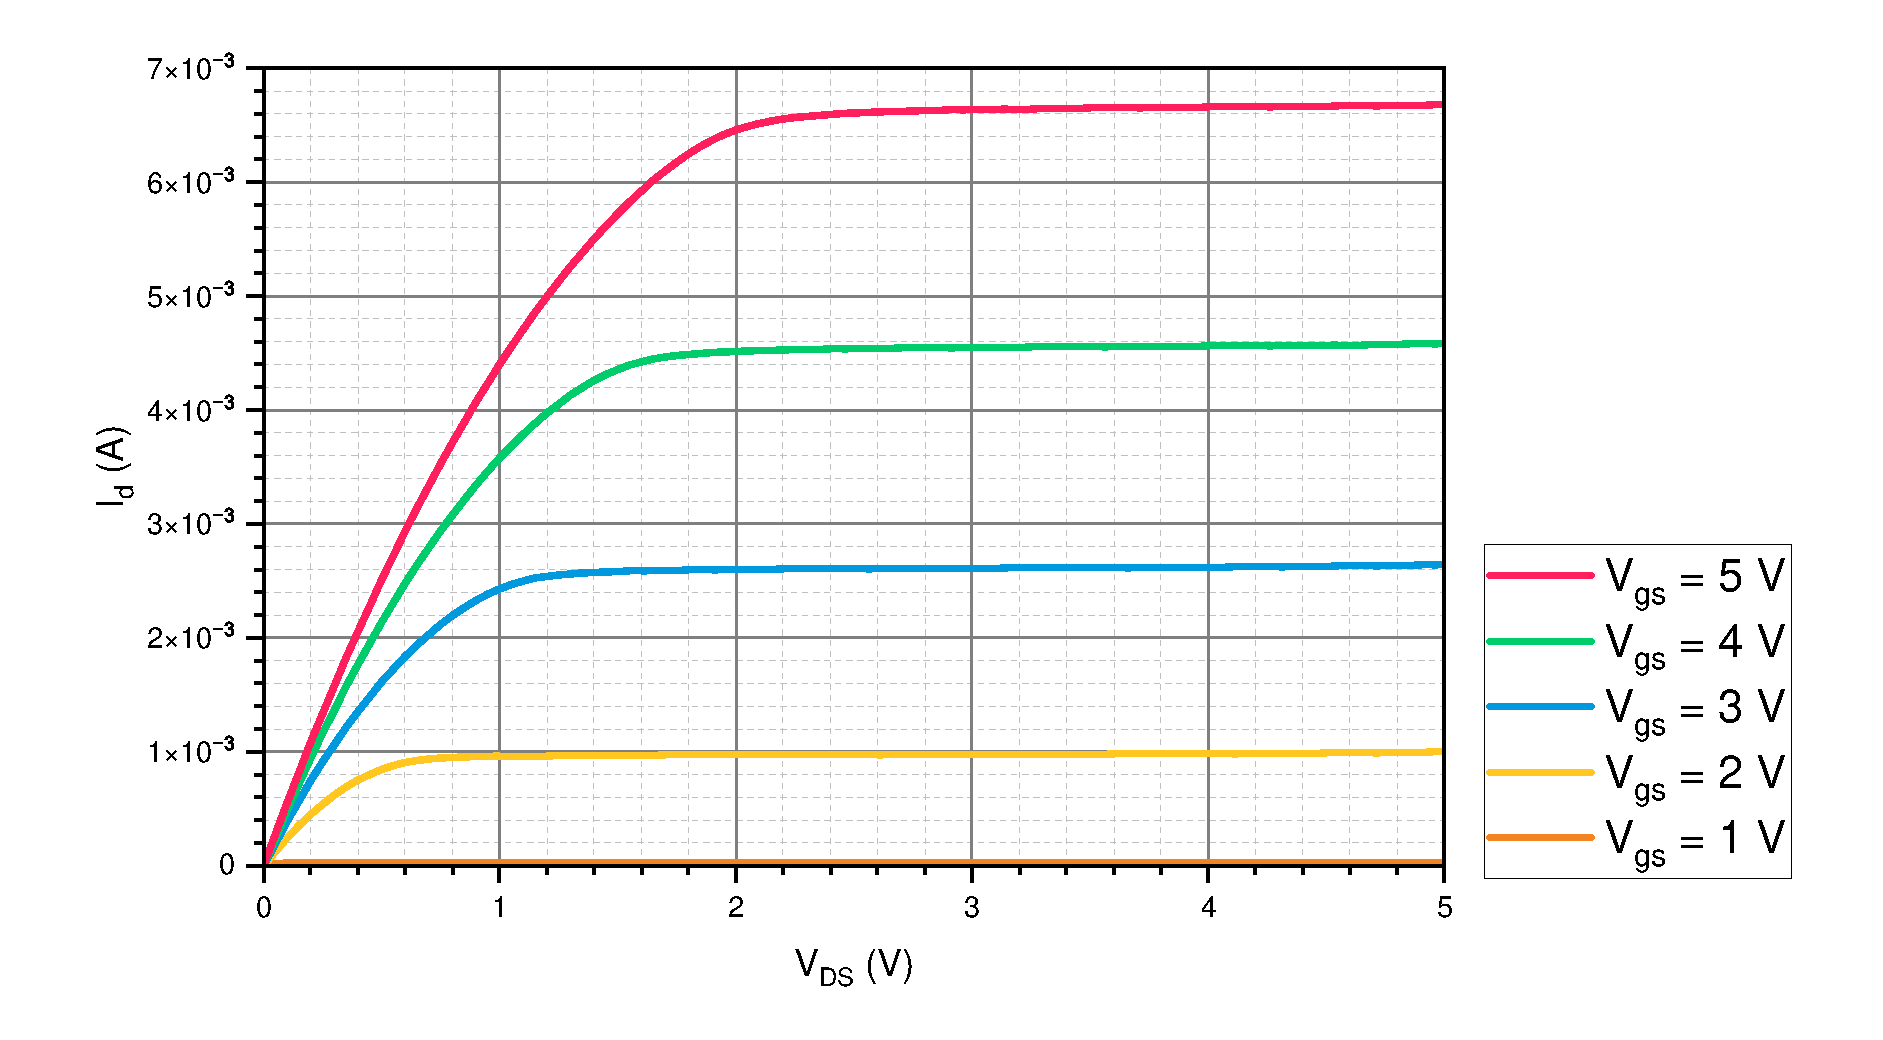
\includegraphics[width=0.7\linewidth]{Figures/E1_NMOS_Characteristic/Group_Id_VDS}
		\caption{The plot of $I_d$ against $V_{DS}$ under 5 different $V_{GS}$}
		\label{fig:groupIdVds}
	\end{figure}
	
	Considering the plot which $V_{GS} = \SI{2}{\volt}$, the curve in the saturation region could be expressed as equation \eqref{eq:idsSat}. The parameter $\lambda$ in the equation is used to model the channel-length modulation effect of the transistor.
	\begin{equation}
		I_{DS} = \beta \left(V_{GS} - V_{T}\right)^2 \left(1 + \lambda V_{DS}\right)
		\label{eq:idsSat}
	\end{equation}
	Substitute two groups of $V_{DS}$ and $I_{DS}$ and take the ratio of them:
	\begin{equation}
		\frac{I_{DS1}}{I_{DS2}} = \frac{9.781 \times 10^{-4}}{9.805 \times 10^{-4}} = \frac{1 + \lambda V_{DS1}}{1 + \lambda V_{DS2}} = \frac{1 + 3\lambda}{1 + 3.5\lambda}
	\end{equation}
	Simplify this equation to get $\lambda = 4.981 \times 10^{-3}\ \si{\per\volt}$. The output resistance of the transistor can be calculated using equation \eqref{eq:outputRes}. 
	\begin{equation}
		r_o = \frac{\delta V_{DS}}{\delta I_{DS}} \approx \frac{1 + \lambda V_{DS}}{\lambda I_{DS}}
		\label{eq:outputRes}
	\end{equation}
	If here we assume that $\lambda V_{DS} \ll 1$, the current $I_{DS}$ is the average current in the range, then substitute the value into equation \eqref{eq:outputRes}:
	\begin{equation}
		r_o \approx \frac{1}{4.981 \times 10^{-3} \times \frac{9.781 + 9.805}{2} \times 10^{-4}} = \SI{205}{\kilo\Omega}
	\end{equation}
	
	Taking $V_{DS} = \SI{5}{\volt}$, the transistor will be saturated for all $V_{GS}$ between $\SI{0}{\volt}$ and $\SI{5}{\volt}$. Figure~\ref{fig:idVgsLinear} shows a plot of $I_{d}$ against $V_{GS}$ simulated under this $V_{DS}$ voltage in linear scale and Figure \ref{fig:idVgsLog} is a plot in log scale.
	
	\begin{figure}[htbp]
		\centering
		\begin{subfigure}{0.48\linewidth}
			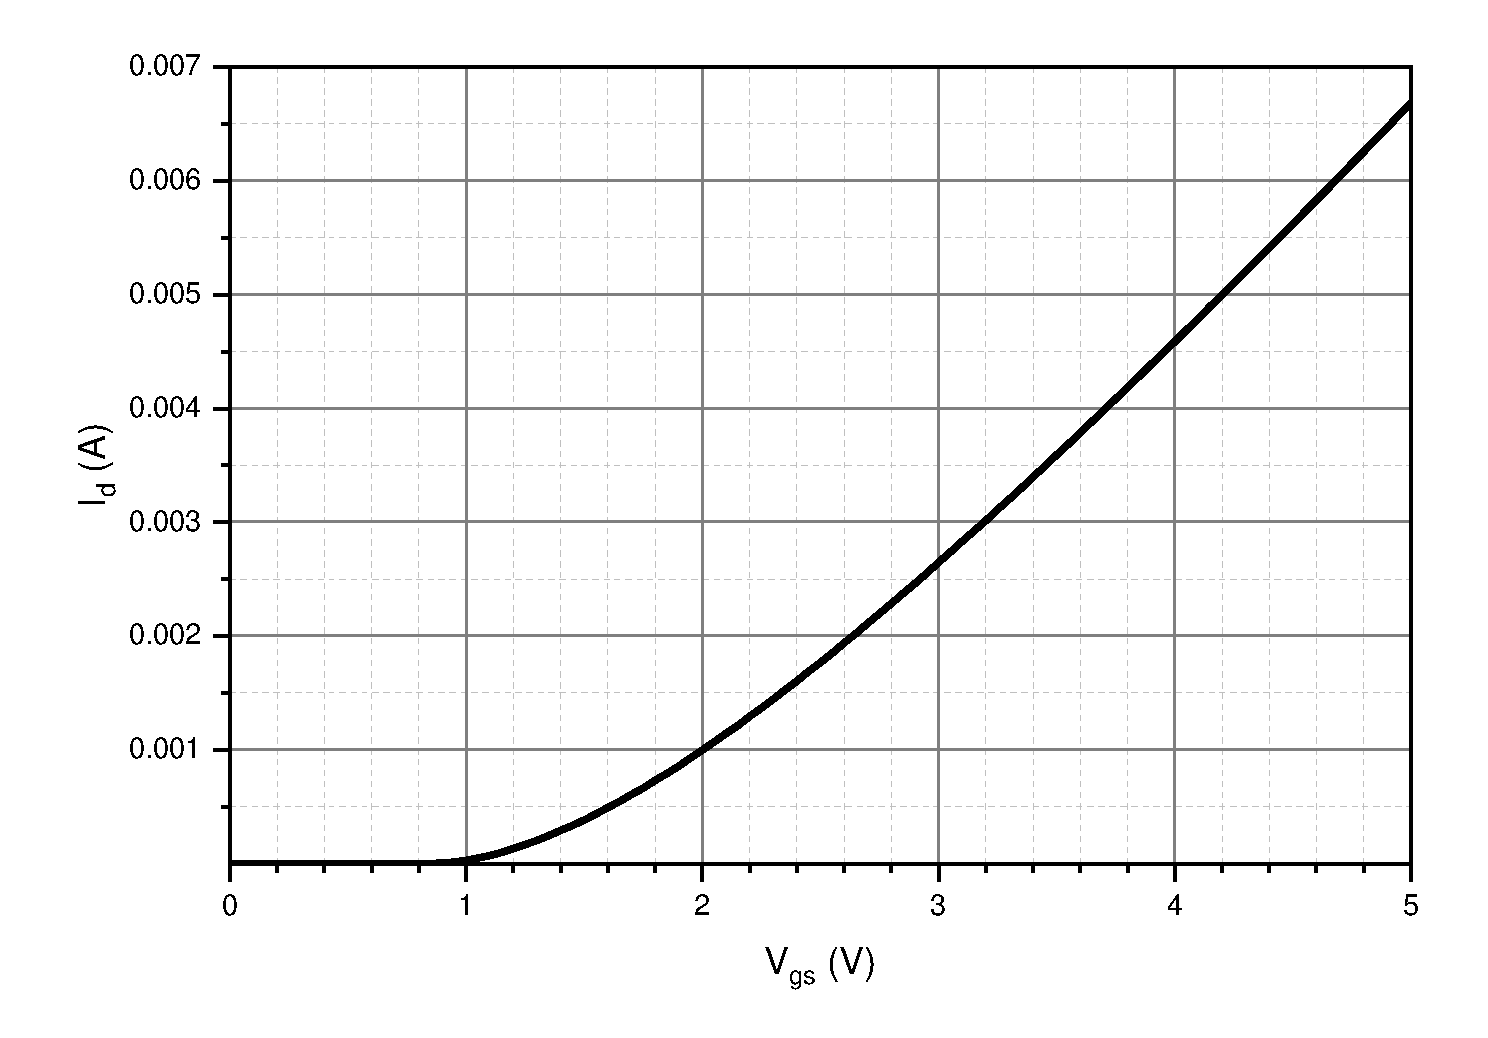
\includegraphics[width=\linewidth]{Figures/E1_NMOS_Characteristic/Id_vgs_linear}
			\caption{}
			\label{fig:idVgsLinear}
		\end{subfigure}
		\begin{subfigure}{0.48\linewidth}
			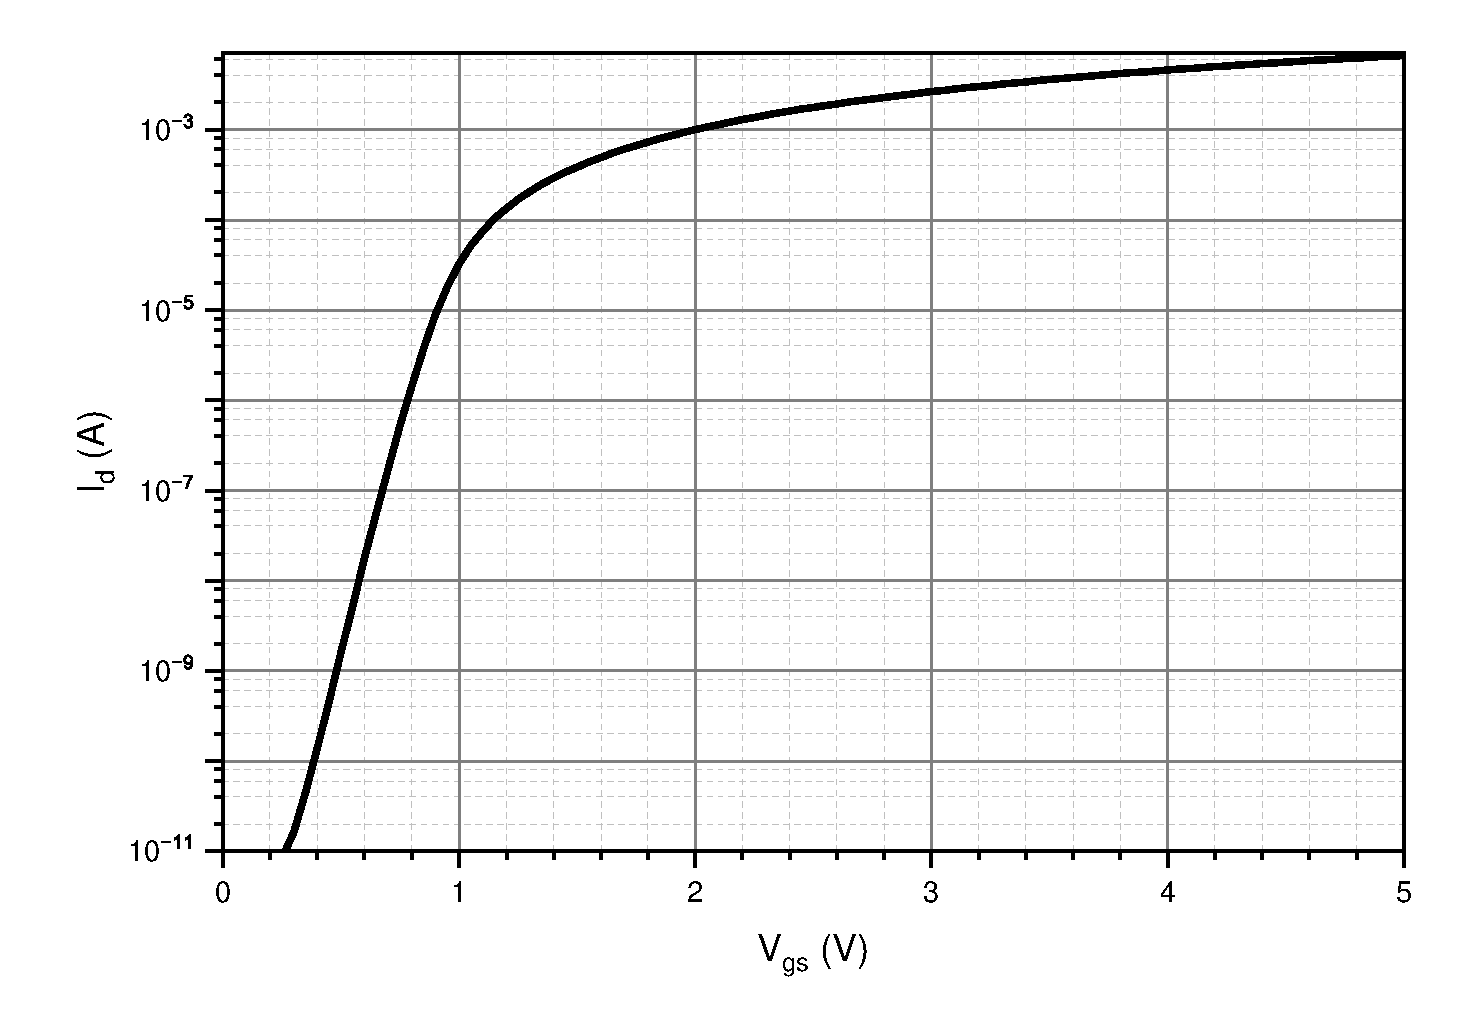
\includegraphics[width=\linewidth]{Figures/E1_NMOS_Characteristic/Id_vgs_log}
			\caption{}
			\label{fig:idVgsLog}
		\end{subfigure}
		\caption{Plot of $I_{D}$ against $V_{GS}$ in (a) linear scale and (b) log scale when $V_{DS} = \SI{5}{\volt}$}
	\end{figure}
	
	The sub-threshold slope is defined as:
	\begin{equation}
		S = \frac{\partial V_{GS}}{\partial \left(\log I_D\right)} \approx \frac{\Delta V_{GS}}{\Delta \left(\log I_D\right)}
	\end{equation}
	To get the slope, I choose to substitute in the value of $\log(I_D)$ when $V_{GS} = \SI{0.4}{\volt}$ and $\SI{0.8}{V}$:
	\begin{equation}
		S \approx \frac{0.8 - 0.4}{-5.835 - \left(-9.852\right)} = 99.6 \times 10^{-3}\ \si{\volt\per\decade}
	\end{equation}
	
	\section{Exercise 2: Common-Source Amplifier}
	
	
	
\end{document}
